\documentclass[english]{scrartcl}
\usepackage[T1]{fontenc}
\usepackage[latin9]{inputenc}

\usepackage{tabularx}
\usepackage{booktabs}

\usepackage{babel}
\usepackage{url}

\usepackage[backend=biber, sorting=none]{biblatex}
\bibliography{references.bib} 

\usepackage{graphicx}

\usepackage{biocon}
\newplant{CS}{genus=Cannabis,epithet=sativa}

\usepackage{xcolor}
\definecolor{mygreen}{rgb}{0,0.6,0}
\usepackage{listings}
\lstdefinestyle{Bash}
{language=bash,
keywordstyle=\color{blue},
basicstyle=\ttfamily,
morekeywords={mkdir,grep,perl,head, makeblastdb, zip, java, blastx, phing,
unzip, screen}, otherkeywords={tbro-db, tbro-import, tbro-tools,
transcripts_to_best_scoring_ORFs.pl, interproscan.sh, RepeatMasker,
rsem-prepare-reference, rsem-calculate-expression, fastq-dump
 } }

\lstdefinestyle{R}
{language=R,
keywordstyle=\color{blue},
basicstyle=\ttfamily,
morekeywords={biocLite,newCountDataSet,estimateSizeFactors, sizeFactors,
counts, normalized, estimateDispersions, plotDispEsts, nbinomTest, plotMA
}, otherkeywords={header} }

\lstset{%
  numbers=none,
  tabsize=3,
  breaklines=true,
  basicstyle=\small\ttfamily,
  framerule=0pt,
  backgroundcolor=\color{gray!25},
  columns=flexible,
  frame=single,
  style=Bash,
  commentstyle=\color{mygreen}\itshape
}

\usepackage{siunitx}


\begin{document}

\title{TBro Manual - Example Dataset}
\author{Markus Ankenbrand}
\maketitle

ERKL\"ARUNG: Hiermit versichere ich, dass ich das vorliegende Protokoll
selbst\-st\"an\-dig verfasst und keine anderen als die angegebenen Quellen und
Hilfsmittel benutzt habe.\\[2cm]

W\"urzburg, \today \hfill Unterschrift

\newpage
\section{Introduction}
The aim of this manual is to teach you how to use the TBro. At first you will
learn how to bring the data into the TBro. For this purpose you can follow the
step by step guide using example data. When you work through this tutorial you
have two options. You can either start from scratch, load the data from the
original sources and perform the analyses yourself or you can just use the
precomputed results in the example directory. In the manual it is assumed that
you perform the analyses yourself so all commands that created the data are
included. However the scope of this manual is not to teach you how to perform
transcriptomic analyses and some of the methods may soon be out of date. The
methods of importing and interpreting the data however will remain the same. If
you choose to use the precomputed data just ignore all commands regarding their
creation and use the accordingly named files in the example directory.

\section{Data}
The demo data consists of the published transcriptome of \plant{CS}. And
additional short read libraries of different samples.

\subsection{Cannabis sativa}
The raw data is available through NCBI. The transcriptome is described
in \cite{CSATIVA} and has accession numbers (JP449145 - JP482359). Read data
from different samples is available through the SRA at NCBI. The used samples
are:
\begin{itemize}
\item Mature flower (SRR306868, SRR306869, SRR306870)
\item Mature leaf (SRR306875, SRR306885, SRR306886)
\item Entire root (SRR306861, SRR306862, SRR306863)
\end{itemize}
We analyzed the data in different ways and final results for each
analysis are included in the example data. You can use this pregenerated results
or generate it yourself, for this purpose each command for data creation along
with program version is given. For an overview of the used programs and versions
see table \ref{tab:PROGRAMS}.

\begin{table}
\caption{Programs used for analyses}
\label{tab:PROGRAMS}
\begin{tabularx}{\textwidth}{Xll}
\toprule
Task & Program & Version\\
\midrule
Peptide prediction & Transdecoder & r2012-08-15\\
Repeat annotation & RepeatMasker & 4.0.3 \\
General annotations & InterproScan & 5 RC5\\
GO/EC annotation & Blast2GO (B2G4Pipe) & 2.5.0\\
General annotation & MapMan (Mercator) & 2013/07/18\\
Count quantification & RSEM & 1.2.5 \\
Normalization / Differential expression & DESeq & 1.12.1 \\
\bottomrule
\end{tabularx}
\end{table}

Data creation and import into TBro is described as a workflow in the next
section.


\section{Bringing the data into TBro}

For this tutorial it is assumed, that you have a fresh install of
TBro as described in the manual \cite{DIP_TBRO}. So you start with a \texttt{CHADO}
database with just a few slight modifications. So lets start populating
the database with our first transcriptome.

\subsection{The Cannabis sativa transcriptome}
\subsubsection{Preparation}
There is one preparation necessary before we can start importing data into TBro.
We have to create the organism as \plant{CS} is not part of the default
\texttt{CHADO} repertoir.
\begin{lstlisting}[style=Bash]
tbro-db organism insert --genus Cannabis --species sativa\
 --common_name Weed --abbreviation C.sativa
 
tbro-db organism list
\end{lstlisting} 
The last command shows us all organisms known to TBro. As we see the ID of
\plant{CS} is 13. We will need this ID for later commands.
You have probably noticed that it is possible to use autocompletion for
commands, subcommands and parameters. In addition the very useful
\texttt{--help} option is present for every command and gives information on
usage, and available parameters.
\subsubsection{The Transcripts}
Create a directory \url{cannabis_sativa} with subdirectory \url{transcriptome} 
\begin{lstlisting}[style=Bash]
mkdir -p cannabis_sativa/transcriptome 
cd cannabis_sativa/transcriptome
\end{lstlisting}
Download the \plant{CS} transcriptome from \texttt{NCBI}. To do so, search for
\texttt{74271[BioProject]} on \url{http://www.ncbi.nlm.nih.gov/nuccore} and
download all hits as fasta. There should be \num{33215} sequences. Save those to
the file \url{cannabis_sativa_transcriptome.fasta} in the newly created folder.
As we have no isoform unigene relationship for those transcripts we treat all
of them as separate isoforms. So the id file comes down to a simple list of all
ids in the fasta.
\begin{lstlisting}[style=Bash]
grep ">" cannabis_sativa_transcriptome.fasta\
 | perl -pe 's/>(\S+).*/$1/'\
 >cannabis_sativa_transcriptome.ids
\end{lstlisting} 
Now, it's time to import the sequence IDs into TBro. As we have no
isoform~-~unigene relationship we import each transcript as a single isoform:
\begin{lstlisting}[style=Bash]
tbro-import sequence_ids --organism_id 13 --release 1.CasaPuKu\
 --file_type only_isoforms cannabis_sativa_transcriptome.ids
\end{lstlisting} 
We had to pass the previously given organism-id and a release name. The release
name can be selected freely and the release is automatically created upon first
usage. The file-type was set to \texttt{only\_isoforms} as we have no unigenes.
Other possible values are \texttt{only\_unigenes} and \texttt{map}. The last
thing we pass is the path to the file containing the sequence-ids which we have
just created.\\
TBro now knows about the sequence ids so lets feed it with the associated
sequences:
\begin{lstlisting}[style=Bash]
tbro-import sequences_fasta --organism_id 13\
 --release 1.CasaPuKu cannabis_sativa_transcriptome.fasta
\end{lstlisting} 
Now it's time to start up your browser and visit your TBro instance. Use the
quick search field in the upper right corner to find
\texttt{gi|351628922|gb|JP481805.1|}. You will see the isoform page with the
basic information about this transcript. By now there is just the general info
(date of import, organism, release) and the sequence together with a
visualization as a horizontal bar. You can check back to this page after every
successful import to watch how the new features are presentet. Of course you can
choose any other isoform that is of interest to you.
\subsubsection{Predicted Peptides}
After we have the nucleotide sequences, the next step is to predict peptides and
load this info into TBro. There are many tools available to predict peptides, we
chose \texttt{Transdecoder} but the TBro does not restrict you to a certain
tool.
\begin{lstlisting}[style=Bash]
mkdir -p ../peptids
cd ../peptids

transcripts_to_best_scoring_ORFs.pl -t \
 ../transcriptome/cannabis_sativa_transcriptome.fasta\
 -m 30 -v --CPU 4 >log >error.log
\end{lstlisting}
Note that we have set the minimum protein length to 30 and number of threads to
4, you can adjust those parameters to your own requirements. Unfortunatelly the
output format for predicted peptides is not standardized. To make the peptide
import generic and not rely on the output format of a special program the import
into TBro is split into two steps. First a list of peptides is imported. This
list has to be in tab delimited format and contain the following columns:
\begin{enumerate}
  \item peptide id
  \item isoform id
  \item start position
  \item end position
  \item strand (+/-)
\end{enumerate}
This file can easily be created from the output of every peptide prediction
program. TBro contains a tool to get the table from the \texttt{Transdecoder}
output so lets use that:
\begin{lstlisting}
tbro-tools transToProt -o predicted_peptides.tbl\
 best_candidates.eclipsed_orfs_removed.pep
\end{lstlisting}
Lets have a look to see that the table has the desired format.
\begin{lstlisting}
head -n5 predicted_peptides.tbl
m.243266        gi|351590686|gb|JP449145.1|     165     893     +
m.243259        gi|351590687|gb|JP449146.1|     1751    1894    +
m.243253        gi|351590687|gb|JP449146.1|     2       1684    +
m.243237        gi|351590688|gb|JP449147.1|     1       1986    +
m.243247        gi|351590688|gb|JP449147.1|     2173    2295    +
\end{lstlisting}
Now to import this peptide table issue the following command:
\begin{lstlisting}
tbro-import peptide_ids --organism_id 13\
 --release 1.CasaPuKu predicted_peptides.tbl
\end{lstlisting}
TBro now knows about the predicted peptides and their locations. What's missing
is the sequences. They are added the same way as the nucleotide sequences of the
transcripts before. It is important, that the fasta IDs exactly match the IDs in
the first column of the peptide table.
\begin{lstlisting}
tbro-import sequences_fasta --organism_id 13\
 --release 1.CasaPuKu best_candidates.eclipsed_orfs_removed.pep
\end{lstlisting}
You might want to check back to the web interface to see our newly imported
peptides.

\subsubsection{RepeatMasker}
Another basic type of annotation are repeats. So we create repeat annotations
using \texttt{RepeatMasker} and import them.  
\begin{lstlisting}
mkdir -p ../analyses/repeats
cd ../analyses/repeats

RepeatMasker -pa 4 -dir . -xm -species viridiplantae\
 ../../transcriptome/cannabis_sativa_transcriptome.fasta
\end{lstlisting}
All we need to do now is tell TBro to import the generated file as \texttt{RepeatMasker}
annotations:
\begin{lstlisting}
tbro-import annotation_repeatmasker --organism_id 13\
 --release 1.CasaPuKu cannabis_sativa_transcriptome.fasta.out.xm
\end{lstlisting}

\subsubsection{Interpro}
\texttt{Interpro} is a usefull tool to annotate protein sequences with information from
different databases. There exists a command line version of this tool called
\texttt{InterproScan}. We use this tool to generate the interpro
annotations for our transcriptome:
\begin{lstlisting}
mkdir -p ../interpro
cd ../interpro

interproscan.sh --pa --iprlookup --goterms --fasta\
 ../../peptids/best_candidates.eclipsed_orfs_removed.pep\
 --output-file-base interpro >interpro.log
\end{lstlisting}
The results in the tsv format can be importet into TBro with the following
command:
\begin{lstlisting}
tbro-import annotation_interpro --organism_id 13\
 --release 1.CasaPuKu -i interproscan-5-RC5 interpro.tsv
\end{lstlisting}
Note that it is important to know the \texttt{InterproScan} version used as each
version uses different versions of the underlying databases. Interpretation of
the results requires knowledge of this versions so the \texttt{-i} switch taking
the version is required for this import.
\subsubsection{Blast2GO}
\texttt{Blast2GO} uses \texttt{BLAST} to find sequence similarities to annotated
sequences. The hits are then used to assign GO terms and EC numbers to the input
sequences.
\begin{lstlisting}
mkdir -p ../blast2go
cd ../blast2go

blastx -query ../../transcriptome/cannabis_sativa_transcriptome.fasta\ 
 -db /path/to/databases/NCBI/nr -evalue 1e-3 -outfmt 5\ 
 -num_alignments 250 -num_descriptions 250\
 -out cannabis_sativa_transcriptome.nr.xml\
 2> cannabis_sativa_transcriptome.nr.log

java -Xmx20G -cp *:ext/*: es.blast2go.prog.B2GAnnotPipe\
 -in cannabis_sativa_transcriptome.nr.xml\
 -out cannabis_sativa_transcriptome.blast2go.annot\
 -prop b2gPipe.properties -v -annot -dat -img\
 > cannabis_sativa_transcriptome.blast2go.log
\end{lstlisting}
First all sequences are blasted against a local copy of \texttt{nr}. The output
format is set to 5 (xml output). The e-value cutoff was set to $10^{-3}$.
Afterwards the \texttt{BLAST} output is passed to the \texttt{Blast2GO} annotation
pipeline.
We can extract three different kinds of annotations from the \texttt{Blast2GO}
output:

\paragraph{GO}
Gene Ontology
\begin{lstlisting}
grep "GO:" cannabis_sativa_transcriptome.blast2go.annot\
 >cannabis_sativa_transcriptome.blast2go.annot.go

tbro-import annotation_go --organism_id 13\
 --release 1.CasaPuKu cannabis_sativa_transcriptome.blast2go.annot.go
\end{lstlisting}
The lines containing ``GO:'' are selected and imported into TBro as
annotation\_go

\paragraph{EC}
Enzyme Commission
\begin{lstlisting}
grep "EC:" cannabis_sativa_transcriptome.blast2go.annot\
 >cannabis_sativa_transcriptome.blast2go.annot.ec

tbro-import annotation_ec --organism_id 13\
 --release 1.CasaPuKu cannabis_sativa_transcriptome.blast2go.annot.ec
\end{lstlisting}
The lines containing ``EC:'' are selected and imported into TBro as
annotation\_ec

\paragraph{Description}
\quad
\begin{lstlisting}
perl -ane 'print if(@F>2)'\
 cannabis_sativa_transcriptome.blast2go.annot.go\
 >cannabis_sativa_transcriptome.blast2go.annot.go.description

tbro-import annotation_description --organism_id 13 --release 1.CasaPuKu\
 cannabis_sativa_transcriptome.blast2go.annot.go.description
\end{lstlisting}
Descriptions are arbitrary text that describes a transcript. Some GO Terms
contain a meaningful description so we import the lines containing such a
description into TBro. However this is just an example, the source of the
description does not matter. The format is a tab delimited format with the
feature ID in the first column and the description in the second.

\subsubsection{Mercator}
Mercator is a tool to classify sequences into MapMan functional plant categories. 
\begin{lstlisting}
mkdir -p ../mercator
cd ../mercator
\end{lstlisting}
To perform the Mercator classification start up your browser and go to
\url{http://mapman.gabipd.org/web/guest/mercator}.\\
In the web interface you can
upload the \texttt{cannabis\_sativa\_transcriptome.fasta}. Unfortunatelly, there
is a restriction on the input file size. This limit is exceeded by our
transcriptome. So you can either contact the people at MapMan to allow you the
submission of a larger dataset or just split the input file into two parts.
We split the file by sequence length but you can just as well open the file
in a text editor and split it. Then run Mercator on each chunk and download the
results afterwards. It is no problem to import the two reports, one after the
other:
\begin{lstlisting}
tbro-import annotation_mapman --organism_id 13\
 --release 1.CasaPuKu mercator.results_max1499.txt
 
tbro-import annotation_mapman --organism_id 13\
 --release 1.CasaPuKu mercator.results_min1500.txt
\end{lstlisting}

\subsubsection{Expression Counts}
Now we have all kinds of annotation for each transcript in the TBro so we can
start with the fun part. Expression data and differential expression data in
particular are the main prospects why we perform RNASeq experiments. So go ahead
and download the SRA files listet above.
\begin{lstlisting}
mkdir -p ../../samples
cd ../../samples

/path/to/sratoolkit/bin/fastq-dump *
\end{lstlisting}
In the samples directory we now have a \texttt{.fq} file for each downloaded
\texttt{.sra} file. The SRA files are no longer required so you can delete them
to save some space. The next step is the quantification by mapping the reads
onto the transcripts. This quantification is done separately for each sample in
the for loop:
\begin{lstlisting}
rsem-prepare-reference cannabis_sativa_transcriptome.fasta\
 cannabis_sativa_transcriptome

for SAMPLE in *.fq
do
BASE=$(basename $SAMPLE .fq)
rsem-calculate-expression -p 4 $SAMPLE cannabis_sativa_transcriptome\
 $BASE >$BASE.log 2>$BASE.err
done
\end{lstlisting}
The results for each sample are aggregated into a single large table with the
perl script \texttt{aggregator\_Count.pl}.
\begin{lstlisting}
perl aggregator_CountMat.pl --in_RSEM\
 SRR306868.isoforms.results SRR306869.isoforms.results\
 SRR306870.isoforms.results SRR306875.isoforms.results\
 SRR306885.isoforms.results SRR306886.isoforms.results\
 SRR306861.isoforms.results SRR306862.isoforms.results\
 SRR306863.isoforms.results\
 --labels_RSEM Flower.mature_L1 Flower.mature_L2 Flower.mature_L3\
 Leaf.mature_L1 Leaf.mature_L2 Leaf.mature_L3\
 Root.entire_L1 Root.entire_L2 Root.entire_L3\
 --out rsem_aggregated.mat
\end{lstlisting}
The resulting table could be imported into
TBro as it is. However the data is not normalized yet. You should always(!)
normalize your expression data. One way to do that is using the \texttt{DESeq}
\texttt{R}-package provided by \texttt{Bioconductor}. So fire up \texttt{R} and
install \texttt{DESeq} if you don't already have it. As we use \texttt{DESeq}
also to create the differential expression data we will already do that and use
the results in the next section.

\begin{lstlisting}[style=R]
# installing and loading DESeq
source("http://bioconductor.org/biocLite.R")
biocLite("DESeq")
library(DESeq)
# loading the expression data
cmat <- read.table(file="rsem_aggregated.mat", row.names=1, header=T)
cond <- sub("_L.*","",colnames(cmat))
# TMM normalization
cds <- newCountDataSet(round(cmat),cond)
cds <- estimateSizeFactors(cds)
write.table(file="rsem_aggregated_TMM.mat", counts(cds,normalized=T),
 quote=F, sep="\t")

# differential expressions
cds <- estimateDispersions(cds)
res.FvsR <- na.omit(nbinomTest(cds,"Flower","Root"))
res.FvsL <- na.omit(nbinomTest(cds,"Flower","Leaf"))
res.RvsL <- na.omit(nbinomTest(cds,"Root","Leaf"))
write.csv(res.FvsL, file="rsem_aggregated_TMM_diff_FvsL.mat", quote=F) 
write.csv(res.FvsR, file="rsem_aggregated_TMM_diff_FvsR.mat", quote=F)
write.csv(res.RvsL, file="rsem_aggregated_TMM_diff_RvsL.mat", quote=F)
\end{lstlisting}

So now we have the expression counts in the file
\texttt{rsem\_aggregated\_TMM.mat}. This file just lacks the header for the
first column so we add it with the following command:
\begin{lstlisting}
sed -i '1{s/^/ID\t/}' rsem_aggregated_TMM.mat
\end{lstlisting}

Before we can go ahead and import the data into TBro we have to make some
preparations. Normally RNASeq experiments are performed on biomaterials in
different conditions. To differentiate between biological signals and random
noise it is mandatory to have replicates for each condition. Each replicate is
called a sample. This hirarchical structure of biomaterial $\rightarrow$
condition $\rightarrow$ sample is also represented in the TBro. So lets tell
TBro about our samples:

\begin{lstlisting}
# Prepare database for Expression Data Import
# Add missing biomaterials (Flower and Root are already present)
tbro-db biomaterial insert --name Flower
tbro-db biomaterial insert --name Leaf
tbro-db biomaterial insert --name Root

# Add conditions
tbro-db biomaterial add_condition --name Flower.mature\
 --parent_biomaterial_name Flower
tbro-db biomaterial add_condition --name Leaf.mature\
 --parent_biomaterial_name Leaf
tbro-db biomaterial add_condition --name Root.entire\
 --parent_biomaterial_name Root

# Add samples
tbro-db biomaterial add_condition_sample --name Flower.mature_L1\
 --parent_condition_name Flower.mature
tbro-db biomaterial add_condition_sample --name Flower.mature_L2\
 --parent_condition_name Flower.mature
tbro-db biomaterial add_condition_sample --name Flower.mature_L3\
 --parent_condition_name Flower.mature
tbro-db biomaterial add_condition_sample --name Leaf.mature_L1\
 --parent_condition_name Leaf.mature
tbro-db biomaterial add_condition_sample --name Leaf.mature_L2\
 --parent_condition_name Leaf.mature
tbro-db biomaterial add_condition_sample --name Leaf.mature_L3\
 --parent_condition_name Leaf.mature
tbro-db biomaterial add_condition_sample --name Root.entire_L1\
 --parent_condition_name Root.entire
tbro-db biomaterial add_condition_sample --name Root.entire_L2\
 --parent_condition_name Root.entire
tbro-db biomaterial add_condition_sample --name Root.entire_L3\
 --parent_condition_name Root.entire
\end{lstlisting}

Also the experiments and analyses should be traceable. So we also have to
include information about the experiment and the different steps in the
analysis. Also the person who performed the analyses has to be specified:

\begin{lstlisting}
# Add contact
tbro-db contact insert --name TBroDemo --description 'TBro Demo User' 
# New item ID is 5.

#Add experiments 
tbro-db assay insert --name SRX082027 --operator_id 4
# New item ID is 1.

# Add acquisitions (corresponding to experiments)
tbro-db acquisition insert --name SRX082027 --assay_id 1
# New item ID is 1.

# Add analyses 
tbro-db analysis insert --name RSEM_TMM --program RSEM\
 --programversion 1.2.5 --sourcename Mapping\
 --description 'RSEM quantification with subsequent TMM normalization'
# New item ID is 50.
tbro-db analysis insert --name DESeq_isoform --program DESeq\
 --programversion 1.12.1 --sourcename Mapping_isoform
# New item ID is 51.

# Add quantifications
tbro-db quantification insert --name RSEM_SRX082027\
 --acquisition_id 1 --analysis_id 50
# New item ID is 1.
\end{lstlisting}

So we have created a contact, assay, acquisition, quantification and two
analyses. Warning: It is important to use the right IDs. Those may differ in
your case so carefully watch the output of each command and note the ID given.
If you forget an ID you can always have a list of all available entries by
issuing:
\begin{lstlisting}
tbro-db <subcommand> list
\end{lstlisting}
After a lot of groundwork we are finaly there. Import the expression counts with
this command:
\begin{lstlisting}
tbro-import expressions -o 13 -r 1.CasaPuKu -q 1 -a 50\
 rsem_aggregated_TMM.mat
\end{lstlisting}

\subsubsection{Differential Expression}
Differential expression is the comparison of the expressions in two different
conditions. When calculating differential expressions statistical methods are
applied to correct for the multiple testing problem. We have already performed
this analysis in the previous section. So if you have skipped the Expression
section you have to use the R snippet there. We also already created the
biomaterials, conditions, analyses, etc. Therefor we can go ahead and import the
differential expression results:
\begin{lstlisting}
tbro-import differential_expressions -o 13 -r 1.CasaPuKu --analysis_id\
 51 -A Flower.mature -B Leaf.mature rsem_aggregated_TMM_diff_FvsL.mat
tbro-import differential_expressions -o 13 -r 1.CasaPuKu --analysis_id\
 51 -A Flower.mature -B Root.entire rsem_aggregated_TMM_diff_FvsR.mat
tbro-import differential_expressions -o 13 -r 1.CasaPuKu --analysis_id\
 51 -A Root.entire -B Leaf.mature rsem_aggregated_TMM_diff_RvsL.mat
\end{lstlisting}

\subsubsection{Blast DB}
To search the transcriptome by homology. Lets add a blast database. To do so we
create a nucleotide database and a protein database and zip them:
\begin{lstlisting}
makeblastdb -in cannabis_sativa_transcriptome.fasta -dbtype nucl
makeblastdb -in cannabis_sativa_predpep.fasta -dbtype prot
zip cannabis_sativa_transcriptome.zip cannabis_sativa_transcriptome.fasta*
zip cannabis_sativa_predpep.zip cannabis_sativa_predpep.fasta*
md5sum *.zip 
# b2ab466c7bfb7d41c27a89cf40837fb4  cannabis_sativa_predpep.zip
# 1f87bbeee5a623e6d2f8cab8f68c9726  cannabis_sativa_transcriptome.zip
\end{lstlisting}
This zip files should now be moved in a location where it can be reached from
the worker machines. To tell TBro about the \texttt{BLAST} databases you should
issue the following command in yout main TBro directory:
\begin{lstlisting}
phing queue-install-db
\end{lstlisting}
This will create a file called \texttt{queue\_config.example.sql} in the current
directory. Rename it to
\texttt{queue\_config.sql} and adjust the appropriate sections like this:
\begin{lstlisting}[language=SQL]
...

-- database files available. name is the name it will be referenced by, md5 is the zip file's sum, download_uri specifies where the file can be retreived
INSERT INTO database_files
 (name, md5, download_uri) VALUES
 ('cannabis_sativa_transcriptome.fasta', '1f87bbeee5a623e6d2f8cab8f68c9726',
 'http://yourdomain/location/cannabis_sativa_transcriptome.zip'),
 ('cannabis_sativa_predpep.fasta', 'b2ab466c7bfb7d41c27a89cf40837fb4',
 'http://yourdomain/location/cannabis_sativa_predpep.zip');

-- contains information which program is available for which program.
-- additionally, 'availability_filter' can be used to e.g. restrict use for a organism-release combination
INSERT INTO program_database_relationships
 (programname, database_name, availability_filter) VALUES
 ('blastn','cannabis_sativa_transcriptome.fasta', '13_1.CasaPuKu'),
 ('blastp','cannabis_sativa_predpep.fasta', '13_1.CasaPuKu'),
 ('blastx','cannabis_sativa_predpep.fasta', '13_1.CasaPuKu'),
 ('tblastn','cannabis_sativa_transcriptome.fasta', '13_1.CasaPuKu'),
 ('tblastx','cannabis_sativa_transcriptome.fasta', '13_1.CasaPuKu');

...
\end{lstlisting}
You have to specify a location that can be reached by your worker machine. If
you just want to have a single worker on the same machine as the server you can
specify the location in the local file system starting with \texttt{file://}.
To perform the changes run the \texttt{queue\_config.sql} commands in your queue
database.\\
Now TBro knows about the database and shows it in the web interface. To perform
\texttt{BLAST} searches we need a worker to execute them. So create one with
this command:
\begin{lstlisting}
phing queue-build-worker
unzip unix-worker.zip
\end{lstlisting}
Modify the \texttt{config.php} to your needs. Most values should be preconfigured through
your \texttt{build.properties}. After that you can start the worker (preferably in a
screen):
\begin{lstlisting}
screen -S blastworker
./worker.php config.php
\end{lstlisting}
Have fun blasting.

\subsubsection{Synonym / Publication}
Synonyms and publications can be added using the API key and internal name of
your bibsonomy account. The structure of such a command is as follows:
\begin{lstlisting}
tbro-db feature add_synonym -f 555 --synonym 'InterestingTranscript'\ 
 -b '[[publication/1adaa3fb03xxxxxxxxxxxxxaec4cef920/bibsonomy_username]]'
 -u 'bibsonomy_username' -t symbol -k 34a2149d8xxxxxxxxxxxxxxbebd342aa
\end{lstlisting}

\subsubsection{Pathways}
To use TBros pathway feature we have to connect the imported data to
pathways. As of now this connection is made via EC numbers and KEGG pathways. We
have to import two tables containing descriptions for EC and KEGG identifiers in
the simple formatL:
\begin{lstlisting}
<Identifier><TAB><Description>
\end{lstlisting}
Additionally a mapping of which EC occurs in each KEGG pathway is required in
the following format:
\begin{lstlisting}
<EC number><TAB><KEGG ID>
\end{lstlisting}
We collected EC and KEGG information from ENZYME, Interpro
and priam to get the descriptions and mapping. The resulting tables may not be complete
and up to date so you might wish to create your own tables and mapping.
For a quick start you find the three files \texttt{ec\_info.tab},
\texttt{kegg\_info.tab} and \texttt{ec\_kegg\_map.tab}
\begin{lstlisting}
tbro-tools addECInformationToDB ec_info.tab
tbro-tools addPathwayInformationToDB kegg_info.tab
tbro-tools addEC2PathwayMapping ec_kegg_map.tab
\end{lstlisting}

\subsection{Any other transcriptome}
With the description above it should be easy for you to import any transcriptome
that interests you. The only thing that could differ significantly from the
description above is if you have predicted unigenes for your transcriptome. This
is common practice and if you use a de novo transcriptome assembler like
\texttt{Trinity} you will get unigenes with corresponding isoforms. In this case
the main difference is in the first step importing ids. Instead of importing a
plain list of sequence IDs you import a map of the following format:
\begin{lstlisting}
<Unigene ID><TAB><Isoform ID>
\end{lstlisting}
With a separate line for each isoform. The import command would then be:
\begin{lstlisting}
tbro-import sequence_ids --organism_id 14 --release 1.0\
 --file_type map my_new_transcriptome.map
\end{lstlisting} 
Of course you have to adjust the organism\_id and release parameters. The use of
unigenes brings a number of advantages. You can easily find isoforms that belong
to the same unigene as each isoform contains a connection to its parent and on
the unigene page you have a list of all corresponding isoforms. In addition you
can now load expression and differential expression results on unigene level as
well as on isoform level. Many programs like RSEM can readily handle that.

\section{Exploring the imported Data}
\subsection{Feature annotations}
\begin{figure}
\begin{center}
  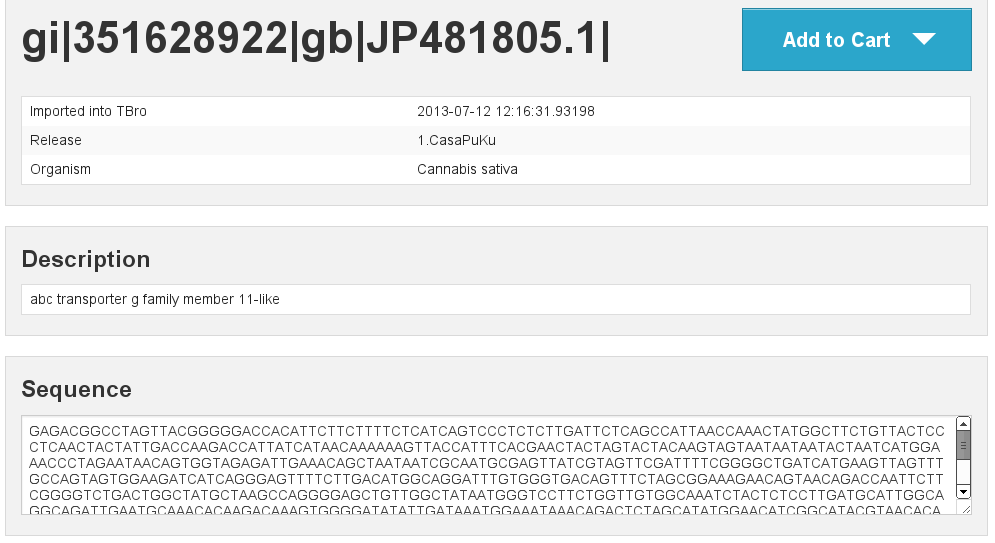
\includegraphics[width=\textwidth]{figures/basic_info.png}
  \caption{Basic information}
  \label{fig:basic}
\end{center}
\end{figure}

\begin{figure}
\begin{center}
  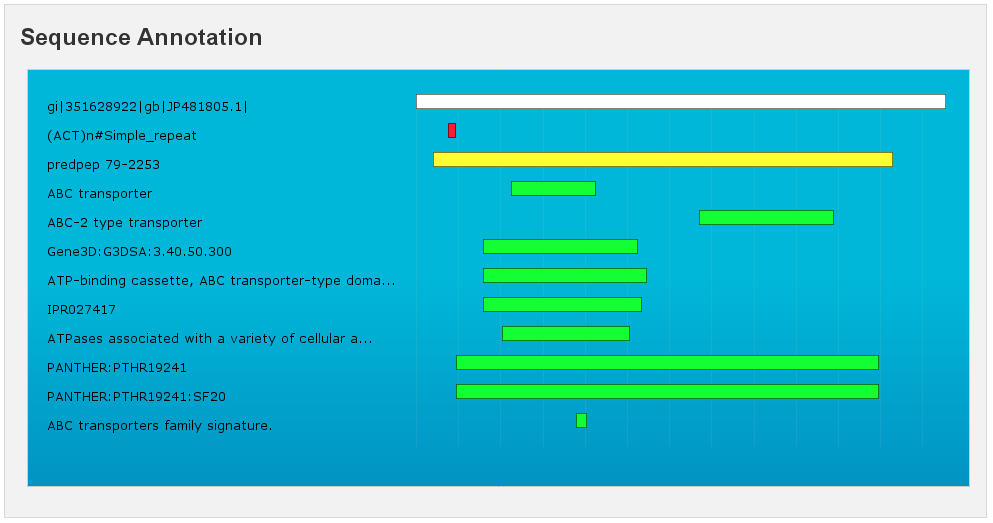
\includegraphics[width=\textwidth]{figures/sequence_annotation.png}
  \caption{Sequence Annotation}
  \label{fig:annotation}
\end{center}
\end{figure}

\begin{figure}
\begin{center}
  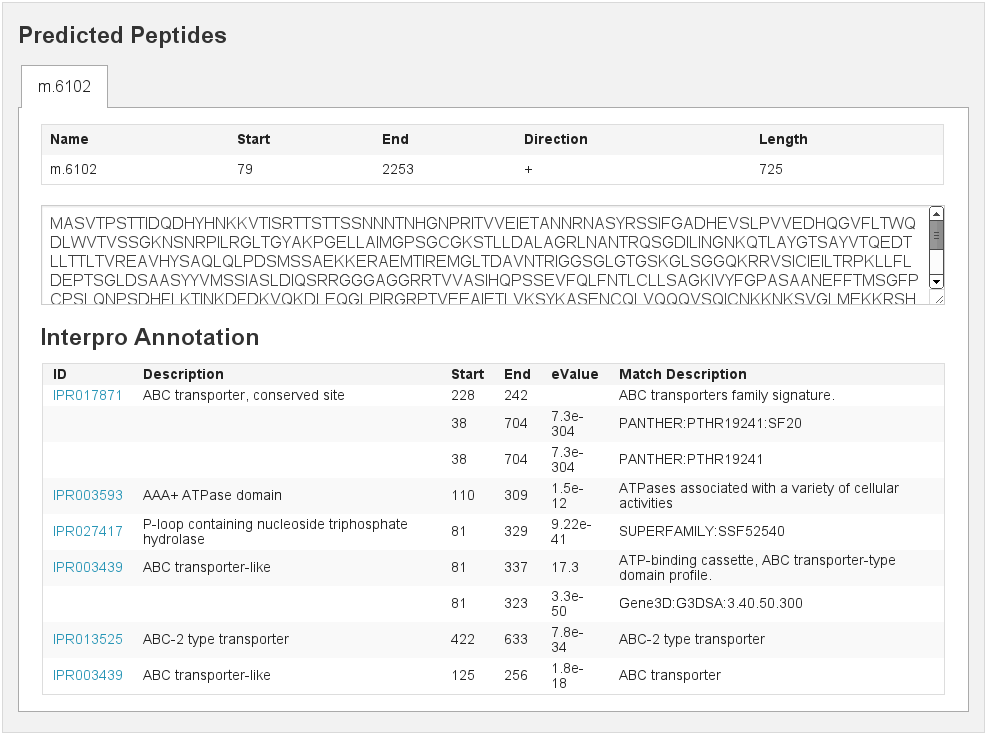
\includegraphics[width=\textwidth]{figures/predicted_peptides.png}
  \caption{Predicted peptids}
  \label{fig:predpep}
\end{center}
\end{figure}

\begin{figure}
\begin{center}
  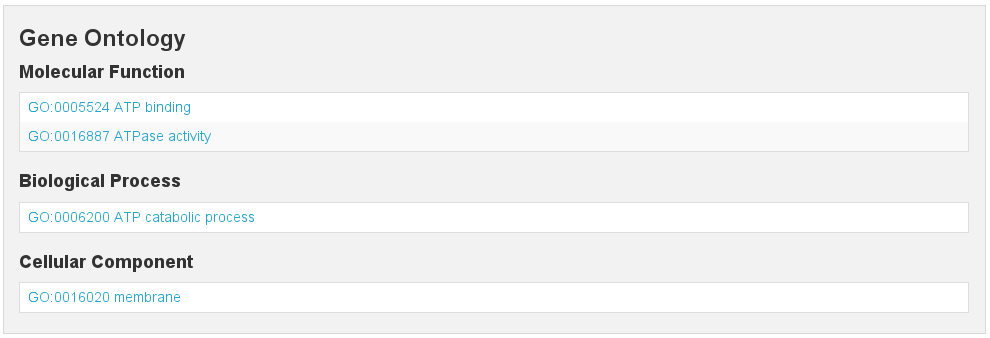
\includegraphics[width=\textwidth]{figures/go.png}
  \caption{GO}
  \label{fig:go}
\end{center}
\end{figure}

\begin{figure}
\begin{center}
  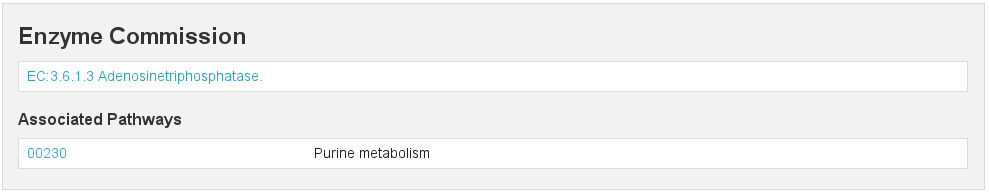
\includegraphics[width=\textwidth]{figures/ec.png}
  \caption{EC}
  \label{fig:ec}
\end{center}
\end{figure}

\begin{figure}
\begin{center}
  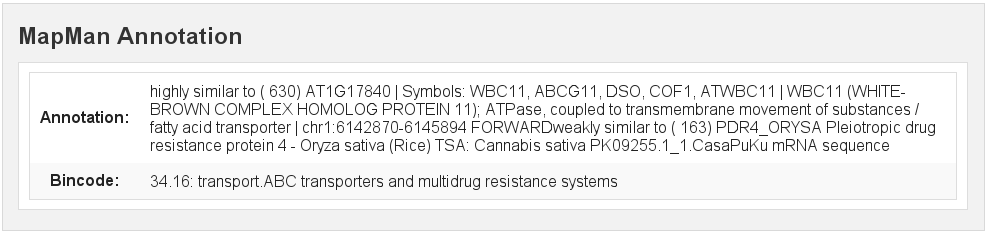
\includegraphics[width=\textwidth]{figures/mapman.png}
  \caption{Mapman Mercator}
  \label{fig:mapman}
\end{center}
\end{figure}

\begin{figure}
\begin{center}
  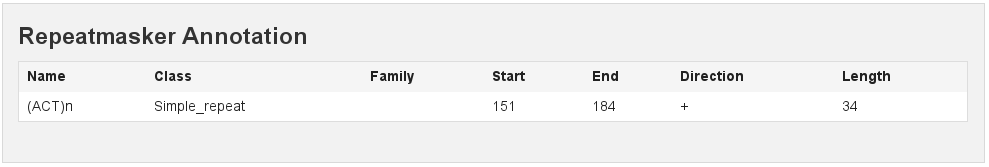
\includegraphics[width=\textwidth]{figures/repeatmasker.png}
  \caption{RepeatMasker}
  \label{fig:repeatmasker}
\end{center}
\end{figure}

\subsection{Expressions}
\begin{figure}
\begin{center}
  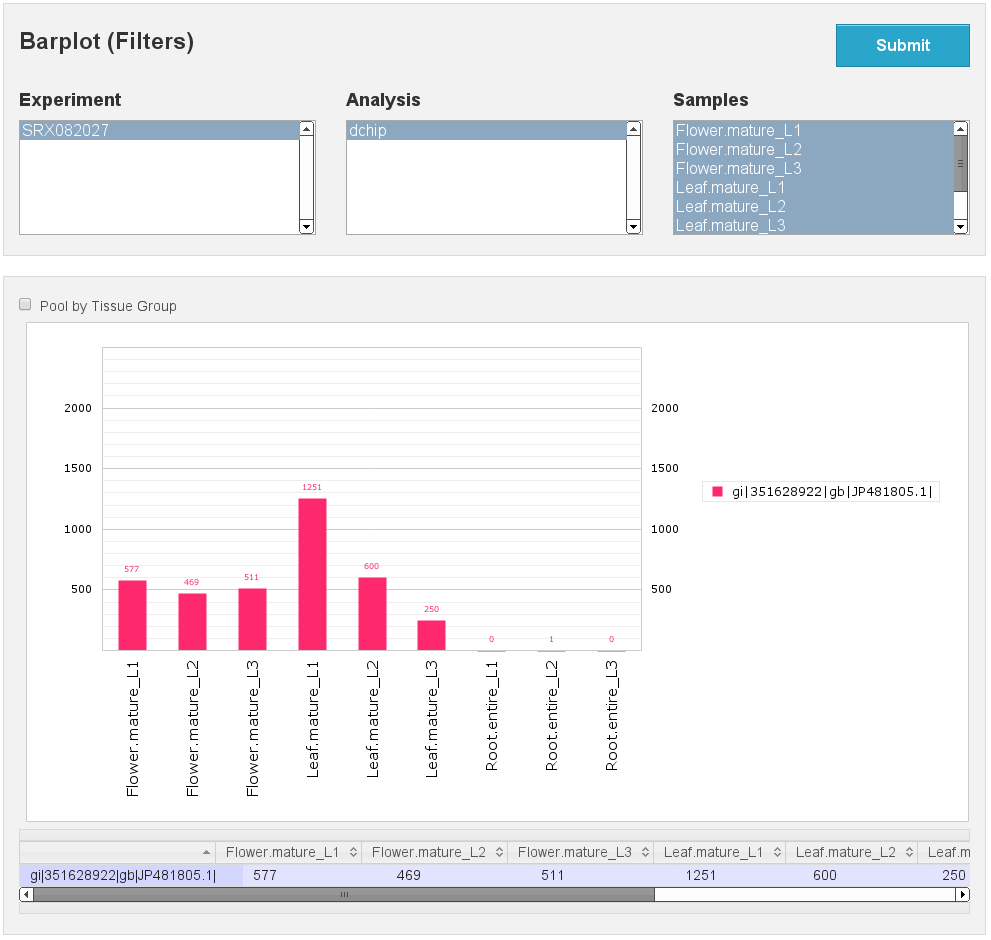
\includegraphics[width=\textwidth]{figures/barplot_iso.png}
  \caption{Expression Barplot for a single Isoform}
  \label{fig:barplot_iso}
\end{center}
\end{figure}
\begin{figure}
\begin{center}
  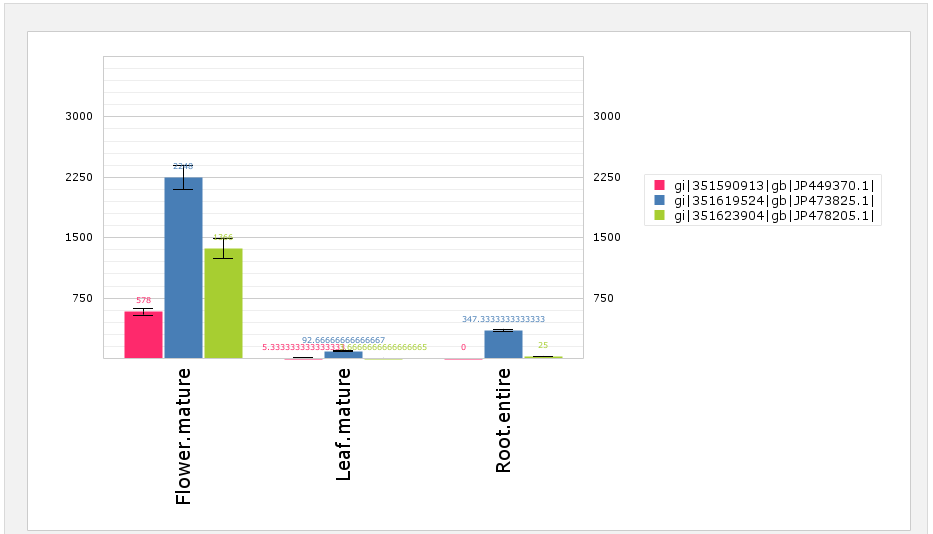
\includegraphics[width=\textwidth]{figures/barplot_cart.png}
  \caption{Expression Barplot for all isoforms in a cart}
  \label{fig:barplot_cart}
\end{center}
\end{figure}

\subsection{Differential Expressions}
\begin{figure}
\begin{center}
  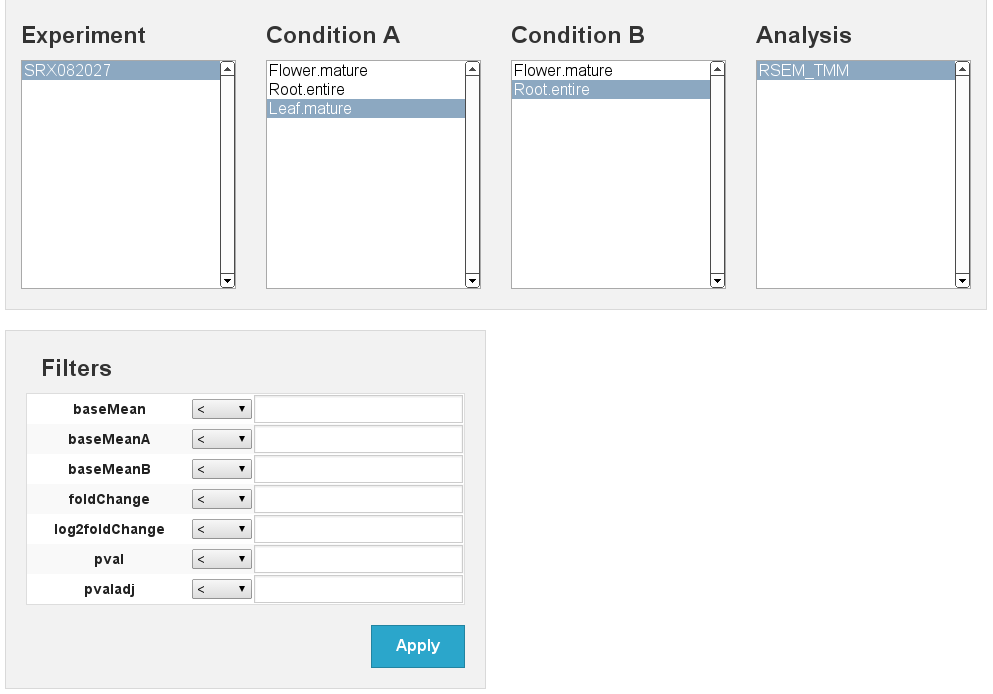
\includegraphics[width=\textwidth]{figures/diffexp.png}
  \caption{Differential expression}
  \label{fig:diffexp}
\end{center}
\end{figure}
\begin{figure}
\begin{center}
  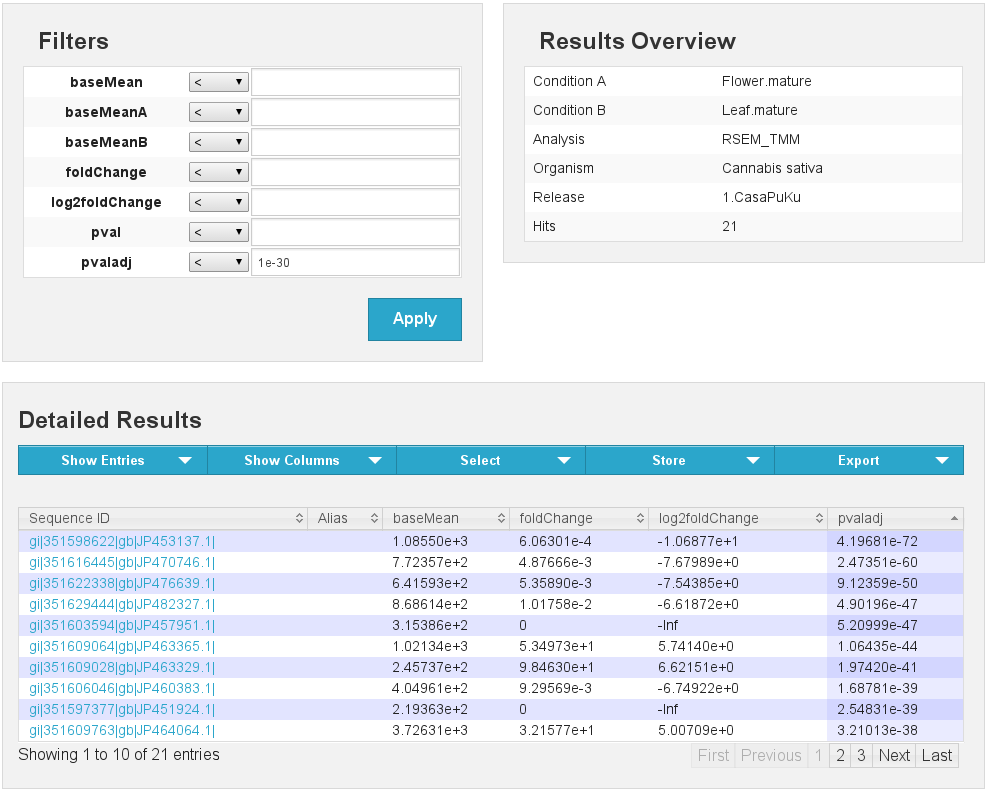
\includegraphics[width=\textwidth]{figures/diffexp_results.png}
  \caption{Differential expression results Flower vs Leaf}
  \label{fig:diffexp_results}
\end{center}
\end{figure}

\subsection{Carts}
\begin{figure}
\begin{center}
  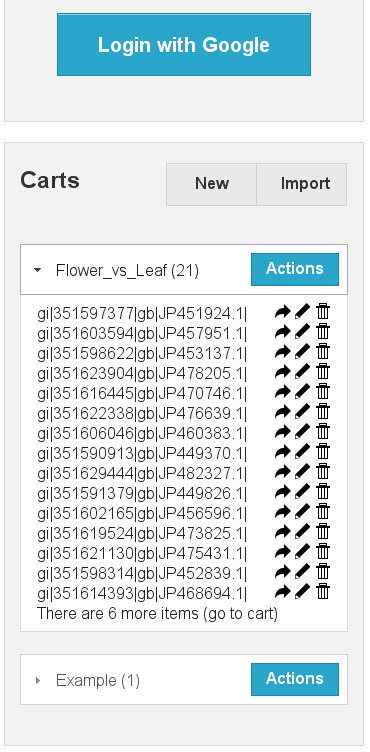
\includegraphics[width=0.5\textwidth]{figures/carts.png}
  \caption{Carts}
  \label{fig:carts}
\end{center}
\end{figure}

\subsection{Pathways}
\begin{figure}
\begin{center}
  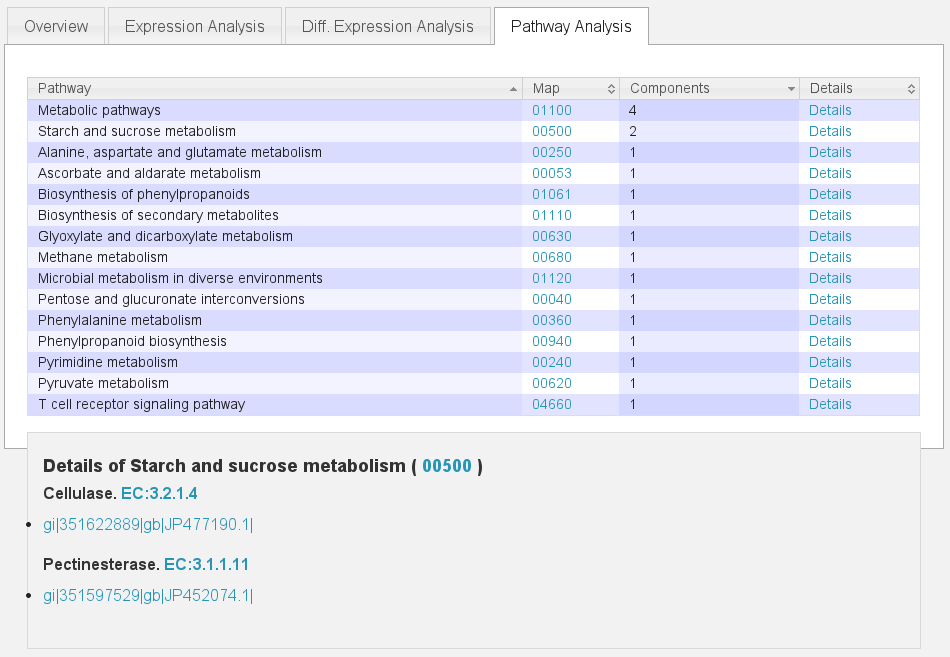
\includegraphics[width=\textwidth]{figures/pathway.png}
  \caption{List of Pathways in the cart}
  \label{fig:pathway}
\end{center}
\end{figure}

\subsection{Searches}
\begin{figure}
\begin{center}
  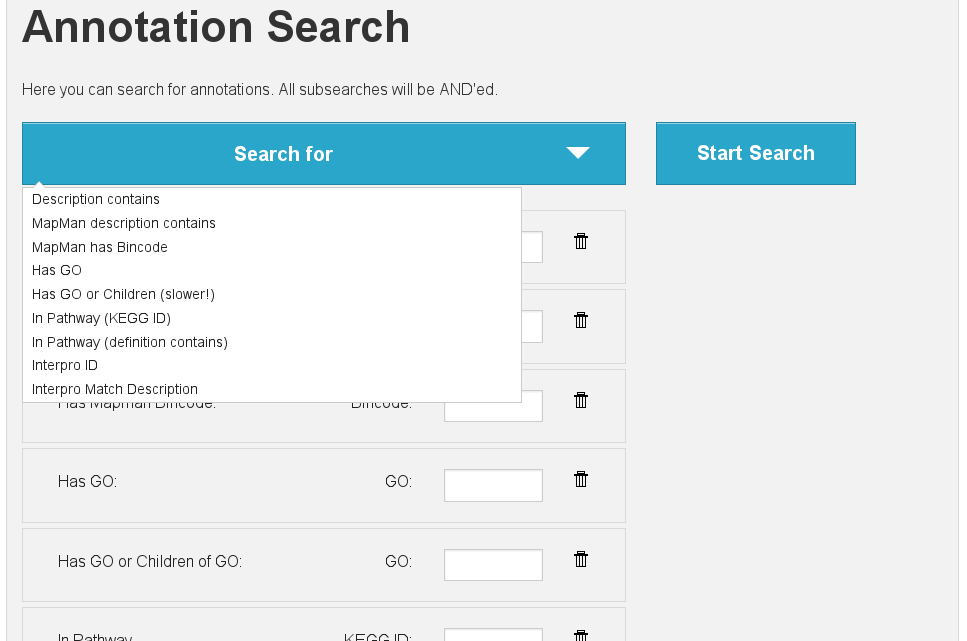
\includegraphics[width=\textwidth]{figures/combisearch.png}
  \caption{Combisearch}
  \label{fig:combisearch}
\end{center}
\end{figure}
\begin{figure}
\begin{center}
  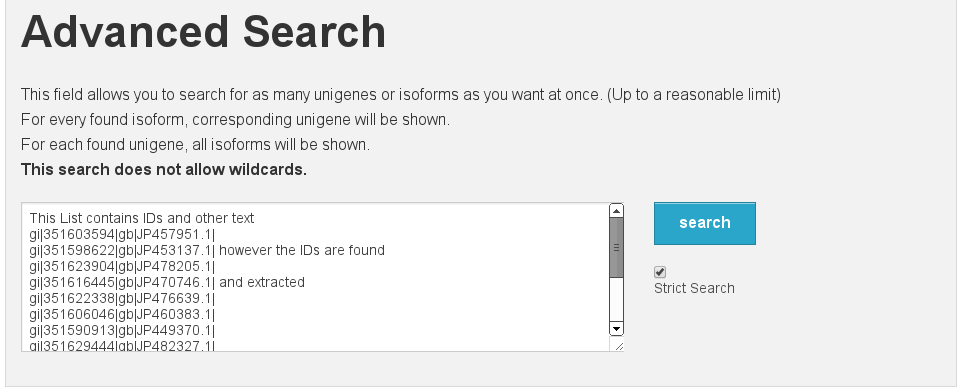
\includegraphics[width=\textwidth]{figures/multisearch.png}
  \caption{Multisearch}
  \label{fig:multisearch}
\end{center}
\end{figure}

\subsection{Blast}
\begin{figure}
\begin{center}
  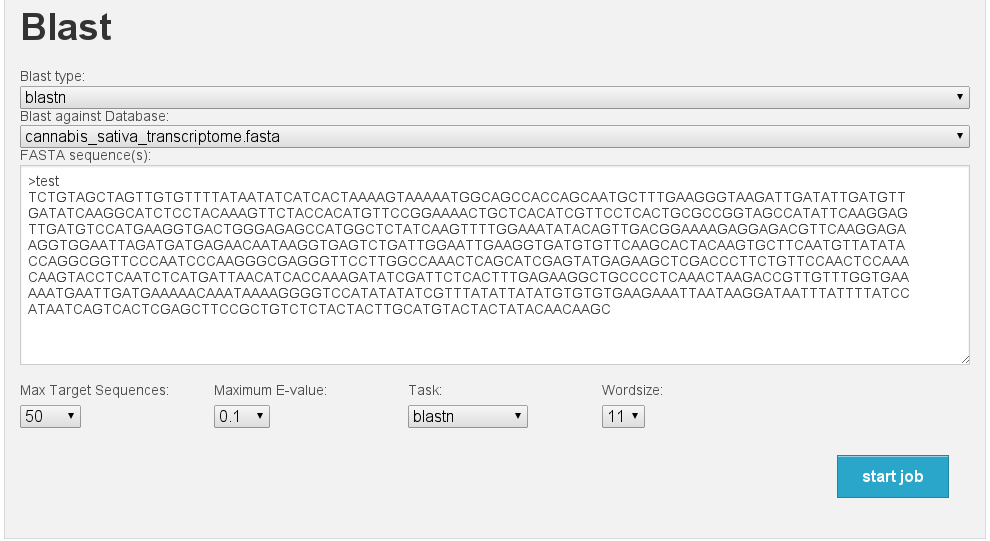
\includegraphics[width=\textwidth]{figures/blast.png}
  \caption{Blast interface}
  \label{fig:blast}
\end{center}
\end{figure}
\begin{figure}
\begin{center}
  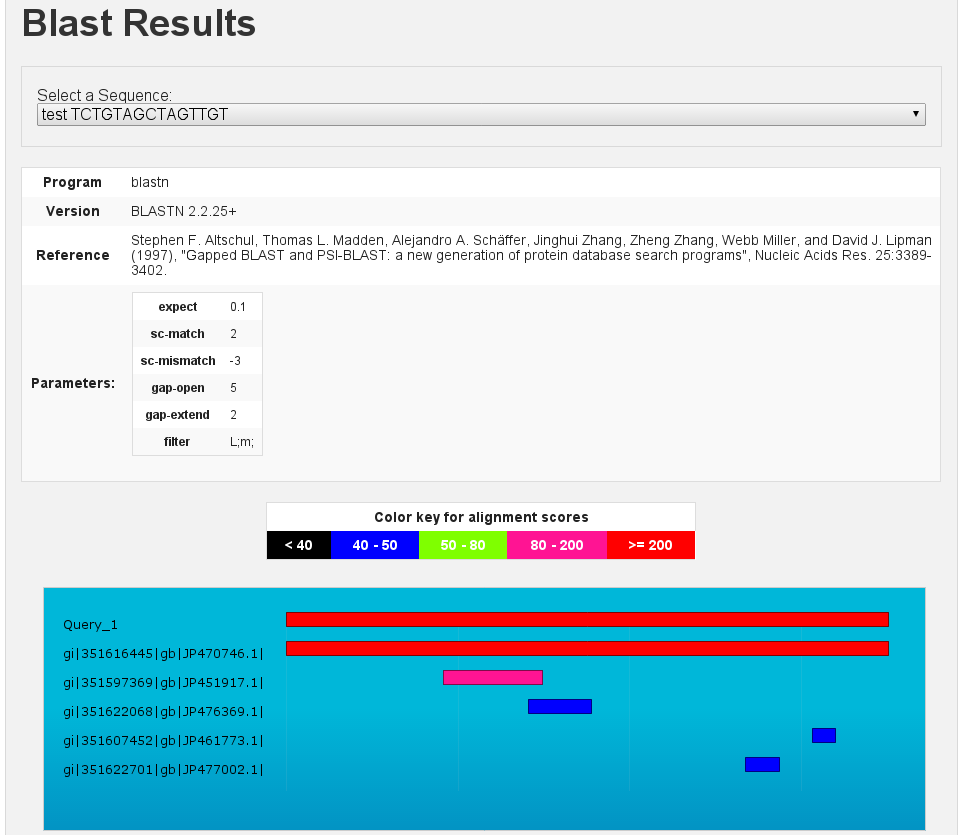
\includegraphics[width=\textwidth]{figures/blast_results_1.png}
  \caption{Blast results}
  \label{fig:blast_results_1}
\end{center}
\end{figure}
\begin{figure}
\begin{center}
  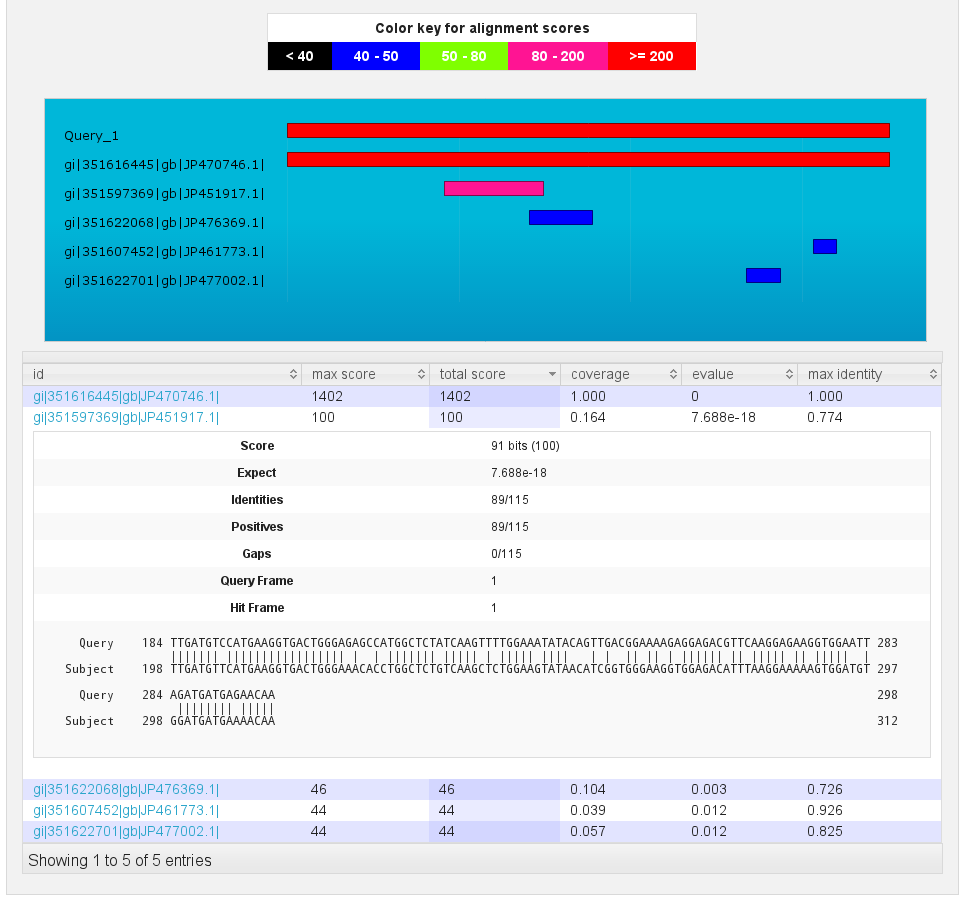
\includegraphics[width=\textwidth]{figures/blast_results_2.png}
  \caption{Blast results}
  \label{fig:blast_results_2}
\end{center}
\end{figure}

\newpage
\section*{}
\printbibliography

\end{document}
